\documentclass[tikz,border=10pt]{standalone}
\usepackage{tikz}
\usetikzlibrary{calc}

\begin{document}
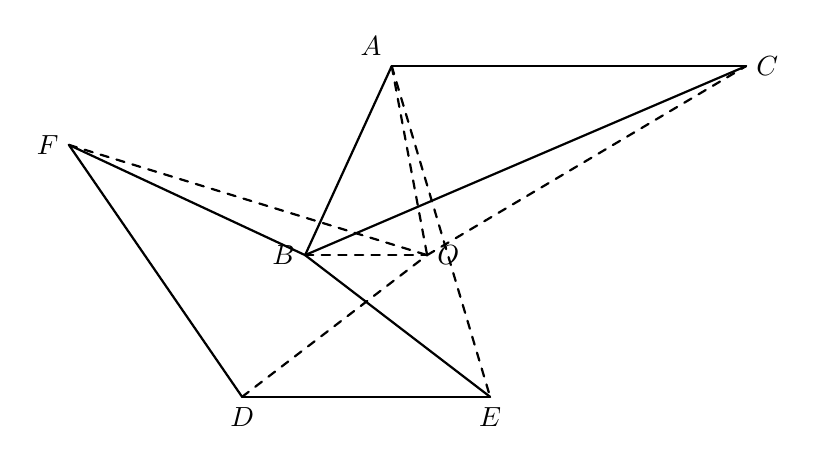
\begin{tikzpicture}[line cap=round,line join=round,thick]

% Coordinates
\coordinate (F) at (0.0,3.2);
\coordinate (B) at (3.0,1.8);
\coordinate (A) at (4.1,4.2);
\coordinate (C) at (8.6,4.2);
\coordinate (O) at (4.55,1.8);
\coordinate (E) at (5.35,0.0);
\coordinate (D) at (2.2,0.0);

% Solid segments
\draw (A) -- (B);
\draw (A) -- (C);
\draw (B) -- (C);
\draw (F) -- (B);
\draw (F) -- (D);
\draw (B) -- (E);
\draw (D) -- (E);

% Dashed segments
\draw[dashed] (F) -- (O);
\draw[dashed] (B) -- (O);
\draw[dashed] (A) -- (O);
\draw[dashed] (O) -- (C);
\draw[dashed] (D) -- (O);
\draw[dashed] (A) -- (E);

% Labels
\node[above left] at (A) {$A$};
\node[left] at (B) {$B$};
\node[right] at (C) {$C$};
\node[right] at (O) {$O$};
\node[below] at (D) {$D$};
\node[below] at (E) {$E$};
\node[left] at (F) {$F$};

\end{tikzpicture}
\end{document}
